%%=============================================================================
%% Methodologie
%%=============================================================================

\chapter{\IfLanguageName{dutch}{Methodologie}{Methodology}}
\label{ch:methodologie}

\section{Inleiding}
Om een antwoord te krijgen op de onderzoeksvraag wordt een experiment opgesteld. Dit experiment zal, per benadering van de verschillende State Management, twee resultaten opleveren. Het eerste resultaat zal het aantal lijnen code van het project bevatten per benadering. Hoe deze meting te werk zal gaan wordt in de volgende sectie besproken. Als tweede resultaat wordt een automatische procedure een aantal keer doorlopen, dit wordt uitvoeriger besproken in \ref{se:prestaties}.

Als eerst worden de nodige voorbereidingen voor dit experiment besproken.

\section{Voorbereidingen}
De layout van de mobiele applicatie is gebasseerd op een mock-up. Deze mock-up werd vooraf gemaakt zodat er tijdens het ontwikkelen van de applicatie geen tijd besteed wordt aan de visuele aspecten. De mock-ups zijn onder deze sectie terug te vinden.

De applicatie heet StoreIt, het hoofddoel van de applicatie is om producten op te lijsten en producten toe te voegen als verkoper. Om de complexiteit van de app te beperken wordt geen onderscheid gemaakt tussen \textit{een klant} en een \textit{een verkoper}. De koper heeft als doel de lijst van product te raadplegen en de details van een product te bekijken. Een verkoper heeft als hoofddoel om een product toe te voegen. In dit experiment worden de klant en de verkoper als eenzelfde gebruiker beschouwd. Er is ook een mogelijkheid om op het voorkeuren scherm het thema van de applicatie in te stellen. De beschikbare thema's zijn een lichte- en donkere modus.
De \textbf{bottom navigation bar} maakt het mogelijk om te navigeren tussen de pagina's. De \textbf{bottom navigation bar} zal ervoor zorgen dat de verschillende schermen worden getoond op de juiste tab. Voor het veranderen van de tab wordt een index bijgehouden om te weten welke tab actief is. Hiervoor wordt \verb|setState()| gebruikt, aangezien er sprake is van een ephemeral state.

\begin{figure}
    \begin{tabular}{cc}
        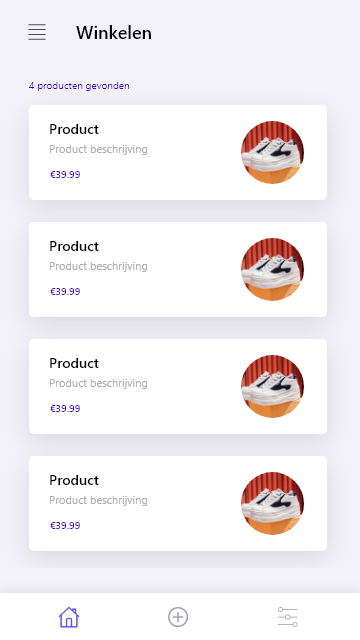
\includegraphics[width=65mm]{img/methodologie/mock-home_screen.png} &   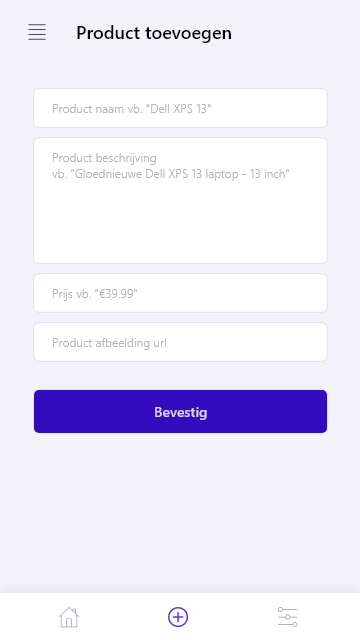
\includegraphics[width=65mm]{img/methodologie/mock-add_product_screen.png} \\
        (a) Mock-up: product lijst scherm & (b) Mock-up: product toevoegen scherm\\[6pt]
        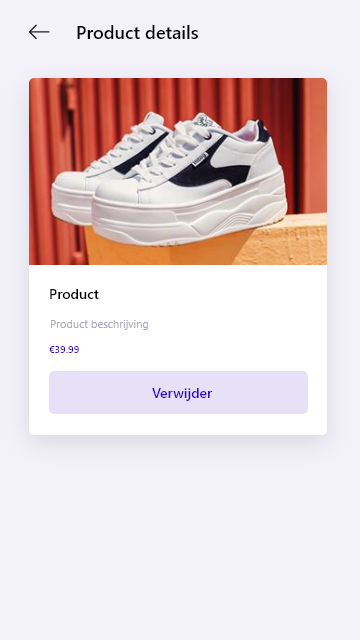
\includegraphics[width=65mm]{img/methodologie/mock-details_screen.png} &   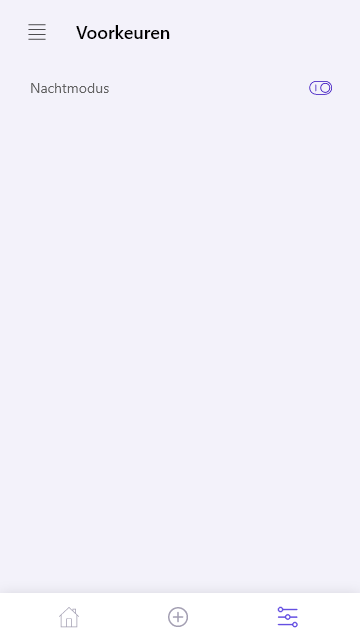
\includegraphics[width=65mm]{img/methodologie/mock-preferences.png} \\
        (c) Mock-up: product details scherm & (d) Mock-up: Voorkeuren scherm \\[6pt]
    \end{tabular}
    \caption{caption}
\end{figure}

\section{Aantal lijnen code}
Om een benaderend meetniveau te verkrijgen voor de complexiteit van een State Management worden de aantal lijnen code geteld. Dit resultaat zal een beeld scheppen op de hoeveelheid code die geschreven moet worden om een benadering van State Management uit te schrijven. Merk op dat de complexiteit van een benadering verschillend is van ontwikkelaar tot ontwikkelaar, dit is en blijft een subjectief meetniveau. Uit dit resultaat wordt besloten hoe rap een benadering van State Management geschreven kan worden. Dit kan leiden tot bijvoorbeeld volgende conclusies: Flutter beginners zullen de voorkeur geven aan benaderingen die vlugger zijn uit te schrijven. 

De aantal lijnen code van de Dart bestanden worden geteld, dit zijn de bestanden met de \verb|.dart| extensie. Hiervoor wordt per verschillende benadering het volgende commando gebruikt: \verb|find . -name '*.cs' | xargs wc -l|. Dit commando geeft het totaal aantal lijnen terug, dit zal per verschillende benadering uitgevoerd worden. Tijdens het schrijven van de benaderingen wordt er rekening gehouden met volgende afspraken: commentaar in de code wordt, vooraleer het commando wordt uitgevoerd, verwijderd. Er wordt enkel gebruik gemaakt van een backspace (nieuwe lijn) voor de scheiding van de verschillende methodes. De afspraken worden strict nagestreefd doorheen de verschillende benaderingen.

\section{Prestaties}
\label{se:prestaties}
\subsection{Integration testen}
Flutter beschikt over de nodige tools voor het uitvoeren van integration testen. Dit zijn testen waarbij de gebruiker-flow van een applicatie wordt gesimuleerd. Deze testen schrijven de gebruiker-flow uit, waardoor individuele modules als één geheel getest kunnen worden. Een integration test bestaat uit de eindapplicatie die ook gebruikt zou worden in productie en een test suite. De test suite definieert de stappen die doorlopen worden tijdens de integration test. Een voorbeeld van een flow: \textit{Gebruiker klikt op een product, vervolgens verwijdert de gebruiker het product...} \autocite{Flutter2019b}. De test suite vindt de nodige widgets in de applicatie door een unieke \verb|key| te definiëren in de broncode. In de test suite wordt dit widget opgeroepen met: \verb|final productItemFinder = find.byValueKey('product-item');|.

Deze integration testen worden gebruikt om de automatische gebruiker-flow uit te schrijven zodat telkens hetzelfde pad wordt doorloopt per benadering van State Management.

Om de effectieve integration testen te schrijven wordt de \verb|flutter_driver| dependency gebruikt.
Een integration test maakt een ``instrumentale'' versie van de applicatie. Deze instrumentale versie maakt het mogelijk om de applicatie te besturen (met de stappen uit de test suite) en prestaties te capteren.
De integration testen worden uitgevoerd in de zogenaamde profile modus van Flutter. De profile modus compileert en start een applicatie bijna identiek als de release mode (voor in productie). De profile modus zorgt enkel en alleen voor de extra functionaliteiten om prestatie problemen te capteren en te debuggen.

\subsection{Gebruiker flow}
De focus van de verschillende benaderingen van State Management worden toegepast op volgende zaken: 
\begin{itemize}
    \item De gebruiker wijzigt het thema op het Voorkeuren scherm.
    \item De gebruiker voegt een nieuw product toe, als gevolg dat de lijst van producten moet bijgewerkt worden op de andere tab.
    \item De gebruiker verwijdert een product op het Product Details scherm, als gevolg dat de lijst van producten moet bijgewerkt worden op de andere tab.
\end{itemize}
Voor deze puntjes zal per benadering te broncode worden aangepast. De broncode van eenbenadering van een State Management wordt gestart vanaf de boiler template code. Deze template wordt op voorhand geschreven. Deze code bevat onder andere de nodige widgets, bijvoorbeeld een product-item, de knoppen...
Bij deze template is geen sprake van State Management, buiten de state van de \verb|BottomNavigationBar|. De verdere State Management wordt aangevuld per verschillende benadering.

De test suite bevat de volgende stappen die chronologisch worden uitgevoerd:
\begin{enumerate}
    \item De gebruiker opent de applicatie en navigeert naar de startpagina
    \item De gebruiker klikt op het laatste product in de lijst
    \item De gebruiker verwijdert het product
    \item De gebruiker navigeert naar de startpagina
    \item De gebruiker navigeert naar het ``voeg product toe'' scherm
    \item De gebruiker vult het formulier in en voegt het product toe
    \item De gebruiker navigeert naar de startpagina
    \item De gebruiker klikt op het nieuwe product
    \item De gebruiker verwijdert het nieuwe product
    \item De gebruiker navigeert naar het ``voorkeuren'' scherm
    \item De gebruiker klikt op de ``nachtmodus'' switch
    \item De gebruiker navigeert naar de startpagina
    \item De gebruiker klikt op een product
    \item De gebruiker verwijdert het product
    \item De gebruiker navigeert naar het ``voeg product toe'' scherm
    \item De gebruiker vult het formulier in en voegt het product toe
    \item De gebruiker navigeert naar de startpagina
    \item De gebruiker sluit de applicatie
\end{enumerate}

% TODO: aanvullen met een video hoe deze stappen eruit zien?

Tijdens het doorlopen van de stappen wordt data gecapteerd. Deze date wordt in Flutter beschouwd als een \verb|Timeline| object. De \verb|Timeline| bevat de ruwe uitvoer van de uitgevoerde stappen. Dit json-bestand kan bekeken worden in \verb|chrome://tracing| en resulteert in een visuele voorstelling van de data te zien op figuur \ref{fig:chrome-tracing-timeline}. Deze uitvoer bevat tal van gemeten waarden. Het CPU-gebruik is voor dit onderzoek de belangrijkste gemeten data.

\begin{figure}[H]
    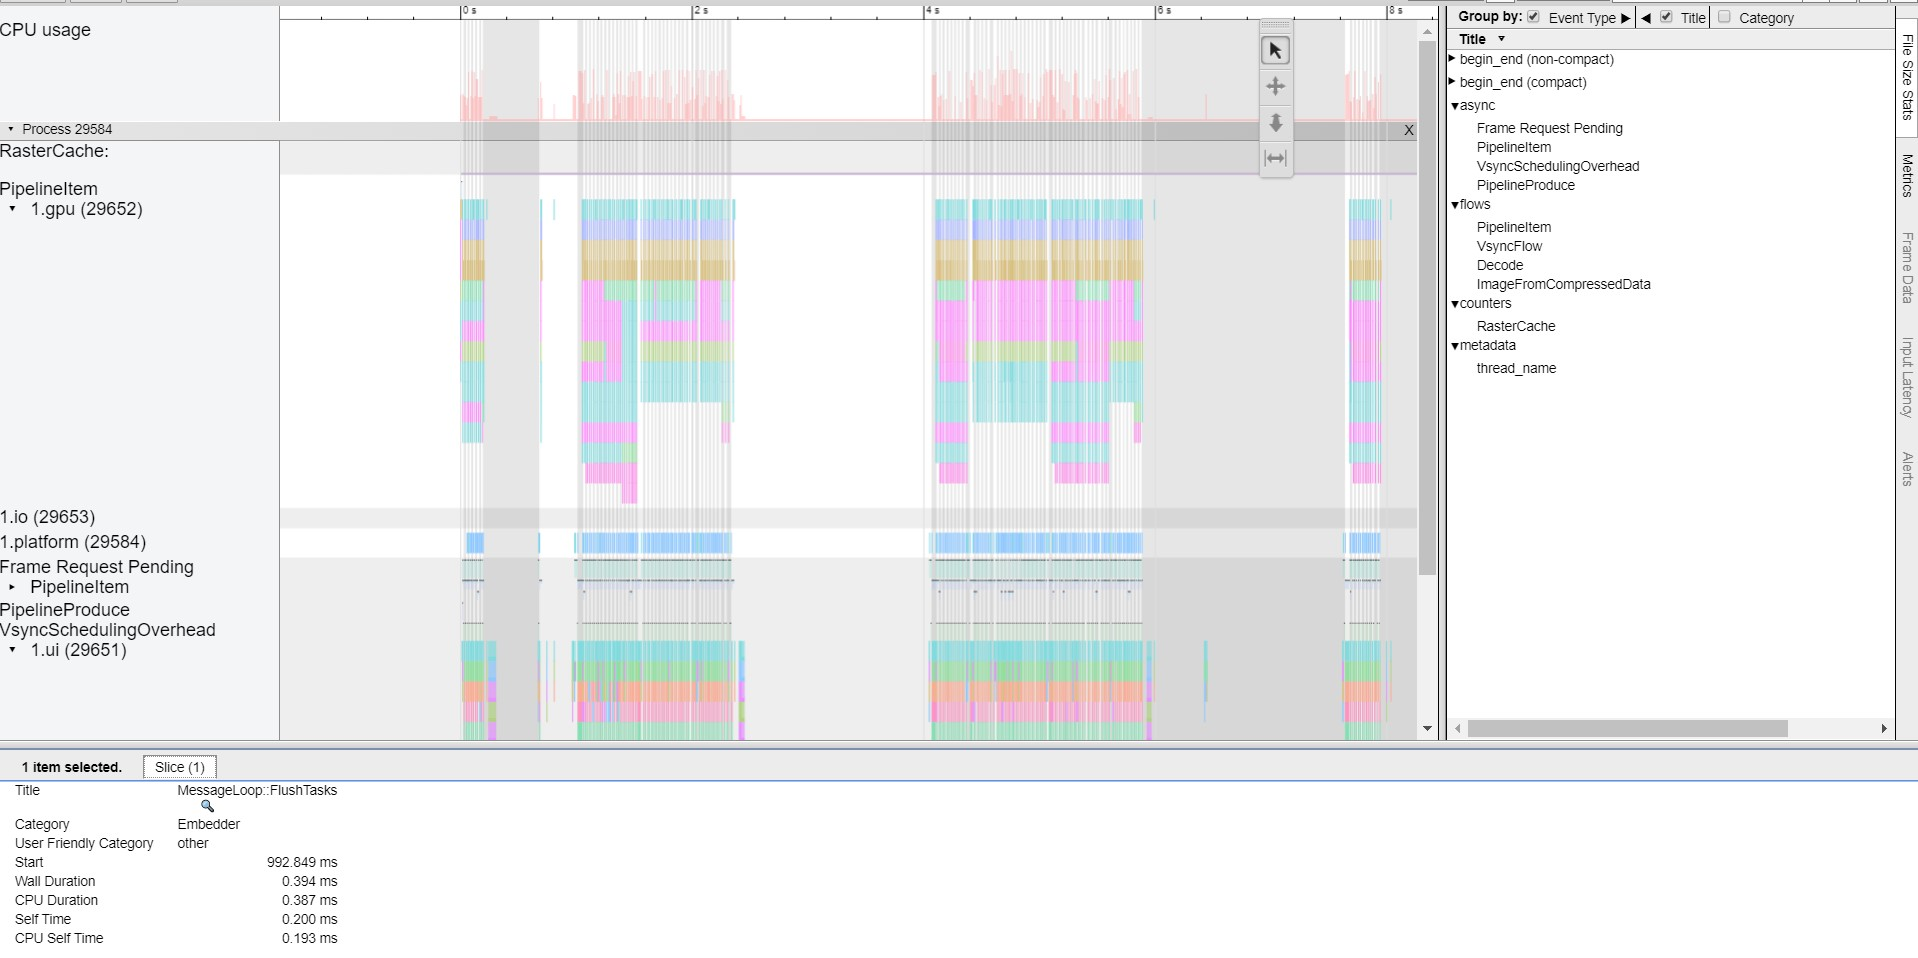
\includegraphics[width=\linewidth]{img/methodologie/chrome-tracing-timeline.jpg}
    \caption{Visuele voorstelling ruwe uitvoer in chrome://tracing}
    \label{fig:chrome-tracing-timeline}
\end{figure}
De stappen worden per benadering doorlopen. Deze procedure zal voor elke benadering dertig keer uitgevoerd worden. 

\subsection{Test apparaat}
Hoewel een iOS Simulator of een Android Emulator goed van pas komen tijdens het ontwikkelen van de applicatie wordt voor het meten van de resultaten beroep gedaan op een echt fysiek apparaat. De meetresultaten van de prestaties die verkregen zouden worden op een emulator zullen verre van een reflectie zijn op de echte wereld. \autocite{Flutter2019c}

Flutter laat het niet toe om de profile modus uit te voeren op een emulator aangezien dit geen steek houdt.
Het test apparaat is een OnePlus 3T zie tabel \ref{table:specifications-test-device} voor de specificaties.
Nadat de broncode is geschreven voor elke State Management benadering en de Flutter integration tests geschreven zijn, kunnen de resulaten verworven worden voor het experiment.

Samengevat worden voor elke bendaring de gegeven stappen doorlopen door middel van de Flutter integration tests. Tijdens deze procedure wordt de verworven data weggeschreven in een json-bestand. Dit json-bevat bevat het nodige om verder te gaan met de analyse van de resulaten.
% TODO: aanvullen? 

\begin{table}[H]
    \centering
    \begin{tabular}{ll}
        Model & A3003 \\
        Besturingssysteem & Android 9.0 - OxygenOS 9.0.6 \\
        Chipset & Qualcomm MSM8996 Snapdragon 821 (14 nm)  \\
        CPU & Quad-core (2x2.35 GHz Kryo \& 2x1.6 GHz Kryo) \\
        GPU &  Adreno 530 \\
        Geheugen & 6GB RAM \\
        Opslag & 64GB \\ 
        &
    \end{tabular}
    \caption{Specificaties van het test apparaat}
    \label{table:specifications-test-device}
\end{table}

%% TODO: Hoe ben je te werk gegaan? Verdeel je onderzoek in grote fasen, en
%% licht in elke fase toe welke stappen je gevolgd hebt. Verantwoord waarom je
%% op deze manier te werk gegaan bent. Je moet kunnen aantonen dat je de best
%% mogelijke manier toegepast hebt om een antwoord te vinden op de
%% onderzoeksvraag.

